\documentclass[titlepage]{article}
\usepackage[left=15mm,right=15mm,top=1in,bottom=1in]{geometry}
\usepackage{framed}
\usepackage{imakeidx}
\usepackage{graphicx}
\usepackage{indentfirst}
\usepackage{array}
\graphicspath{{./img/}}
\newcolumntype{C}[1]{>{\centering\arraybackslash} m{#1cm}}

\makeindex

\title{Autonomous Pool Playing Robot\\~\\\textbf{Proof of Concept}}
\author{
	Ernest Selman\\selmae@mcmaster.ca\\1201291\\~\\\and
	Eric Le Fort\\leforte@mcmaster.ca\\1308609\\~\\\and
	Guy Meyer\\meyerg@mcmaster.ca\\1320231\\~\\\and
	Andrew Danha\\danhaas@mcmaster.ca\\1223881\\~\\\and
	Max Moore\\moorem8@mcmaster.ca\\1320009\\~\\\and
	Derek Savery\\saverydj@mcmaster.ca\\1219142\\~\\
}
 
\begin{document}
\maketitle
\tableofcontents
~\\[15mm]
\listoftables
\listoffigures


\vfill
\begin{table}[!htbp]
\centering
\begin{tabular}{| C{3} | C{2} | C{5} | C{2.5} |}\hline
	Date			&Revision \#	&Comments						&Authors\\\hline
	14/11/2016		&0				&- Initial document creation	&Eric Le Fort\\\hline
	29/11/2016		&1				&- Software section				&Max Moore\newline Eric Le Fort\\\hline
	29/11/2016		&2				&- Hardware section				&Ernest Selman\newline Guy Meyer\newline Andrew Danha\newline Derek Savery\\\hline
\end{tabular}
\caption{Revision History}
\end{table}
\newpage


\section{Introduction}
Throughout this document, various difficult technical components of the automated pool playing robot will be outlined in detail. The document will then address the team's plans to tackle those concerns as necessary.
\subsection{Purpose}
This document will aim to identify and address the most likely sources of failure for this project. Optimally, this document proves that the team is capable of solving these main sources of concern.
\subsection{Acronyms \& Definitions}
A list of all appropriate acronyms and definitions can be found in the requirements document for this project.


\section{Software Proof of Concept}
This section will outline the major software hurdles that must be overcome in order for this project to be a success. For each case, the concern will be discussed followed by the team's plan on how to overcome that issue.

\subsection{Visual Recognition Software Usage}
The system must be able to take a photo of the table and have a program recognize the position of balls. Since no members of our team have previously implemented software capable of achieving this task, it is likely to be a difficult aspect of our design.\\\\
The best way to prove that we are able to overcome this challenge is to make a MATLAB script that is able to locate ball positions. The program written was successfully able to identify and record the position of lightly coloured or well-lit balls. Adding better lighting will solve this problem and moving forward, we are confident that we can recognize stationary balls using image recognition.
\newpage
\begin{figure}
\centering
	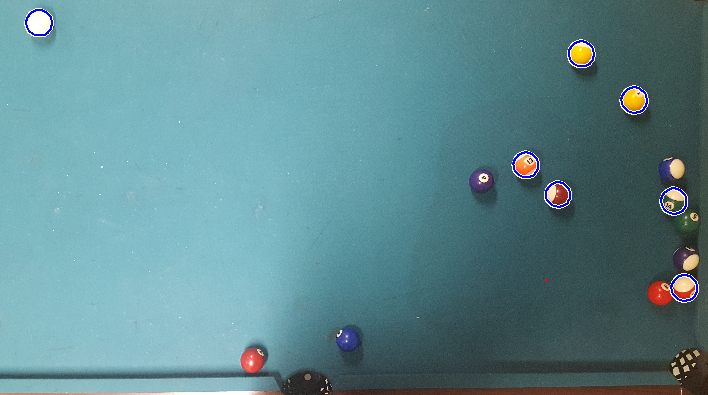
\includegraphics{ballsOnTable.png}
\caption{Results of the VR algorithm.}
\end{figure}~\\

\subsection{Inter-Device Communication}
The system must have a smartphone receive a message wirelessly from the PC and then communicate back an image from the smartphone to the PC.\\\\

This problem can be solved using File Transfer Protocol or the Secure CoPy (SCP) protocol. The request will be sent from the PC to the phone which will then capture an image. Upon completion, the PC will use FTP to receive the photo wirelessly from the computer. Relevant links regarding sources of examples for file transfer from an android to a PC and for file permissions management are provided.\\ 

Android to PC file transfer:\\
http://stackoverflow.com/questions/10417442/client-server-file-transfer-from-android-to-pc-connected-via-socket\\

Hardware to Android file transfer over Wi-Fi:\\
http://stackoverflow.com/questions/20345155/android-receive-and-send-data-through-wifi-connection-to-hardware\\

Using the principles discussed above as well as the tangible examples from the link we are confident we can overcome the problem of device intercommunication.

\subsection{Shot Selection}
Shot selection is likely to be the most challenging aspect of this system from a software perspective. Given a set of possible shot angles, amounts of force, and weighted goals the system would need to simulate a multitude of shots. It is infeasible given the computational time requirements of this system to complete this task using a completely brute force approach.\\

The first piece of the solution to this problem is limiting the granularity of angles to analyze for possible shots. The step size that will be used will be determined as appropriate such that optimal shots are not missed. Furthermore, the step size must be at least the minimum step size of the rotational motor that will aim the end-effector. If it is not possible to take a shot from this angle (e.g. another ball is in the way or the shot is directly into the rails), the algorithm will discard the shot.\\

The algorithm will then simulate taking a shot in that direction at the maximum (100\%) power that the system can safely take. The algorithm will check if the shot causes the cue ball to hit an opponent's ball first, does not hit a ball or sinks the cue ball without hitting a ball. If any of these events are expected to occur, the algorithm will discard the shot.\\

If the shot is not already discarded, certain shot powers will be simulated. This will include an even split somewhere between 4 and 10 of the possible powers (i.e. 25\%/50\%/75\% or 20\%/40\%/60\%/80\%) to be decided based on empirical results later. These shots will be scored based on a number of features such as the robot's balls sunk, opponent balls sunk, if the cue ball was sunk, and so on. The algorithm will go from higher power to lower power. Therefore, if at low power it does not hit a ball, the algorithm can neglect checking lower powers at that shot angle.\\

These logical steps will substantially lower the duration of computation to be made by the algorithm. Our hope is that using this algorithm the duration will be short enough to satisfy the computational time requirement.



\section{Hardware Proof of Concept}
This section will outline the major hardware hurdles that must be overcome in order for this project to be a success. For each case, the concern will be discussed followed by the team's plan on how to overcome that issue.
\subsection{Post-Shot Interference}%TODO
In order to adequately strike a ball anywhere on the table the end-effector or striker will be required to enter the active ball area (the theoretical volume at which object inside it may interfere with a rolling ball). As a result the end-effector must enter this volume to initiate contact with the ball but must not stay inside it much longer to allow the balls to roam freely. Whether it�s a linear or rotational actuator the active motion of exiting the volume must occur.\\

Our team will address this issue by creating a mechanism that will raise the end-effector soon after the shot. This will be done as quickly as possible without damaging the instruments or requiring human intervention to reset it to its striking position. According to current discussions the team is considering a raising motion although we have yet to finalize any designs so the outcome may change if other (and better) solutions arise.
\subsection{Machine State Awareness}%TODO
When the system is required to move from one location to another it will be required to account for the number of steps it needs to move to get there. This is why being able to count the number of steps of all motion motors (linear motor systems for translational motion and rotational motor systems for system orientation) is essential to the success of the project. A difficulty which we may encounter during this project is both the real time tracking of steps and the loss of steps due to disturbances or system error.\\

We will address this issue in several ways. Firstly, the system must be well built in order to not allow slack for the motors to slip or skip steps. Second, we are estimating that most if not all motors will be stepper motors which have a definite mechanical step rather than servos which rely on other tracking methods. We will have a dedicated system within the microcontroller software that will track each step carefully in order to avoid inaccuracies. If the system detects a potential miscalculation there will be known checkpoints that the system will use to calibrate the stepping sequence. These checkpoints are not necessarily often since they are not meant to replace the stepping mechanism of the motor but they should be frequent enough to the program to reset often. The actual number of checkpoints is based on the accuracy of the motor and structure of the system (i.e. an inaccurate system will require lots more checkpoints rather than a very exact solution). I predict somewhere between 2 and 10 checkpoints depending on the integrity of the motion.
\subsection{Recoil from Shots}%TODO
%Should be fine if we build the system sturdy enough. If not a) PID compensator or, b) additional parts to brace when taking a shot
The end-effector will be required to strike at many levels of force in order to score from different positions on the table. Some of the more powerful shots may induce large amounts of recoil in the robotic arm. In order to avoid interfering with the other balls on the table and to avoid damaging the system, the recoil from a shot must be mitigated.\\

To effectively mitigate the recoil of the end-effector, a real-time control system must be implemented. The control system will invoke a force opposite to the recoil of the system in order to maintain the stability of the system.
\subsection{Shot Power Control}%TODO
%Pneumatic will have preset values, if motor, we will send appropriate voltage

Since the system will be required to make shots from most positions on the billiards table, the end-effector must strike at a variable force. After the system takes an image of the table, and processes it through the VR software, it will calculate a vector for the end-effector to strike.\\

Once the system calculates the vector, it will send the distance value to the arduino. Using the distance value, the arduino will then calculate the optimal PWM value to send to the actuator that controls the end-effector's striking motion.
\subsection{Ability to Make All Shots}%TODO
%Mentioned in software -- shot selection. Also the design should aim to require as small of an amount of space to take a shot as possible (to allow shots in tight squeezes)
%No inclusion from their work on purpose, didn't forget to copy. Write from scratch.

\subsection{Sufficient Motor Torque}%TODO
%Add in that we can gear ratio the force if necessary. Two 25N-m motor would cost less than $200
%http://www.omc-stepperonline.com/high-torque-nema-42-cnc-stepper-motor-30nm4248ozin-p-74.html
Due to the nature of the task, the end-effector is required to have a high range of motion while also being highly precise. The implication of these requirements is that the mechanical build of the robot arm will need to be rather extensive, and in effect, could be of considerable weight. Given that the mechanical build could be rather heavy, it is pertinent to consider motor specs required to move the machine.\\

The most pressing concern is specs required to facilitate movement along first dimension of motion (the length of the table most likely) as this will require being able to move the entire weight of the machine.  For our purposes we will use a liberal estimate of 250 kg for the mass of the robot. We will likely be using some form of slide bearing to aid movement of the machine along the first dimension of motion. We will therefore use an estimate of 0.3 for coefficient of static friction (mu). This is, again, a very liberal estimate as coefficient of static friction for slide bearings can vary anywhere from approximately 0.003 to 0.3. Using the mass of the robot and the coefficient of static friction, we find that a force of 250*9.81*0.3 = 735.75 N is required to move the machine along the first dimension of motion.\\

While 735.75 N is a rather high value, it is not entirely unfeasible. It is possible to purchase stepper motors rated for 50 N-m stall torque. This translates to 735.75 N of force at roughly a 6.8 cm effective radius (radius to translate motor rotation to linear motion). As it is likely that we will be using an even smaller radius for this purpose, 6.8 cm is a perfectly acceptable metric. If for some reason a 50 N-m motor is found to be unfeasible it is possible to use multiple motors of lesser capability, two 25 N-m motors for example. Furthermore, intelligent planning with regards to the design of the robot arm could result in a total weight much less than 250kg and the use of high quality slide bearings could result in a coefficient of static friction orders of magnitude less than 0.3. Both of these factors would work to reduce the required stall torque of the motors.
\subsection{Rigid Structure}%TODO
A large portion of the system will include rails which will provide support for translational motion for the end-effector. As a result there must be non-bending bars that will be able to span the long distances of the table. Furthermore all jitter, shaking or unnecessary motion must be reduced in order to provide stability for the system and avoid inaccuracies in the motion.\\

This is will be addressed through the selection of non-flexing materials. These materials will be sturdy and straight at the length required by the design. Additionally, it is planned to apply support points along the way which will ensure straightness if the bar is deemed too long. Finally, the system must be designed to include very little jitter space within connections. All mechanical connections must be tight and be able to withstand disturbances from the environment. 
\end{document}


%Guy: 1,2,7
%Andrew: 3,4
%Ernest: 5
%Derek: 6
